\documentclass[border=5pt]{standalone}
\usepackage{tikz}
\usetikzlibrary{shapes,arrows,positioning}

\begin{document}

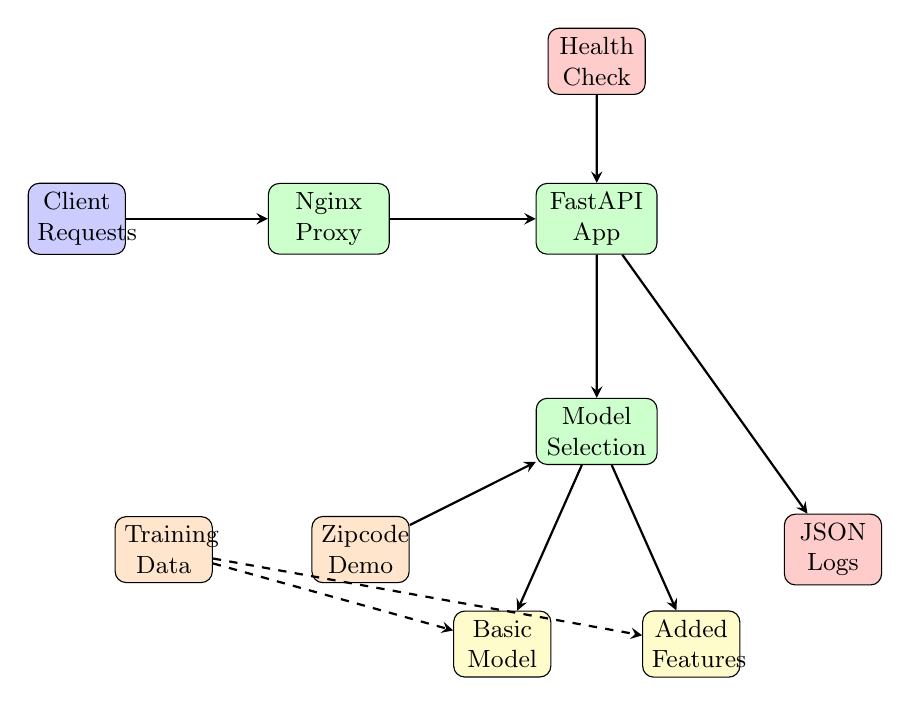
\begin{tikzpicture}[node distance=1.2cm, auto, scale=1.2]
    % Define styles
    \tikzstyle{client} = [draw, rectangle, fill=blue!20, text width=1cm, text centered, rounded corners, font=\small]
    \tikzstyle{service} = [draw, rectangle, fill=green!20, text width=1.3cm, text centered, rounded corners, font=\small]
    \tikzstyle{model} = [draw, rectangle, fill=yellow!20, text width=1cm, text centered, rounded corners, font=\small]
    \tikzstyle{data} = [draw, rectangle, fill=orange!20, text width=1cm, text centered, rounded corners, font=\small]
    \tikzstyle{monitor} = [draw, rectangle, fill=red!20, text width=1cm, text centered, rounded corners, font=\small]
    \tikzstyle{arrow} = [thick, ->, >=stealth]
    
    % Layer 1: Clients
    \node[client] (client) {Client\\Requests};
    
    % Layer 2: Nginx Proxy
    \node[service, right of=client, xshift=2cm] (nginx) {Nginx\\Proxy};
    
    % Layer 3: FastAPI App
    \node[service, right of=nginx, xshift=2.2cm] (fastapi) {FastAPI\\App};
    \node[monitor, above of=fastapi, yshift=0.8cm] (healthcheck) {Health\\Check};
    
    % Layer 4: Model Selection
    \node[service, below of=fastapi, yshift=-1.5cm] (modelsel) {Model\\Selection};
    
    % Layer 5: Models
    \node[model, below of=modelsel, xshift=-1.2cm, yshift=-1.5cm] (basic) {Basic\\Model};
    \node[model, below of=modelsel, xshift=1.2cm, yshift=-1.5cm] (added) {Added\\Features};
    
    % Layer 6: Data Sources
    \node[data, left of=modelsel, xshift=-1.8cm, yshift=-1.5cm] (demographics) {Zipcode\\Demo};
    \node[data, left of=demographics, xshift=-1.3cm] (training) {Training\\Data};
    
    % Layer 7: Logging
    \node[monitor, right of=modelsel, xshift=1.8cm, yshift=-1.5cm] (logs) {JSON\\Logs};
    
    % Arrows: Request flow
    \draw[arrow] (client) -- (nginx);
    \draw[arrow] (nginx) -- (fastapi);
    \draw[arrow] (healthcheck) -- (fastapi);
    \draw[arrow] (fastapi) -- (modelsel);
    \draw[arrow] (modelsel) -- (basic);
    \draw[arrow] (modelsel) -- (added);
    
    % Arrows: Data flow
    \draw[arrow] (demographics) -- (modelsel);
    \draw[arrow, dashed] (training) -- (basic);
    \draw[arrow, dashed] (training) -- (added);
    
    % Arrows: Logging
    \draw[arrow] (fastapi) -- (logs);
\end{tikzpicture}

\end{document}
